\chapter{Program}
\paragraph{}The open-source Arduino Software (IDE) makes it easy to write code and upload it to the board. It runs on Windows, Mac OS X, and Linux. The environment is written in Java and based on Processing and other open-source software. This software can be used with any Arduino board.

\begin{figure}[H]
 \centering
    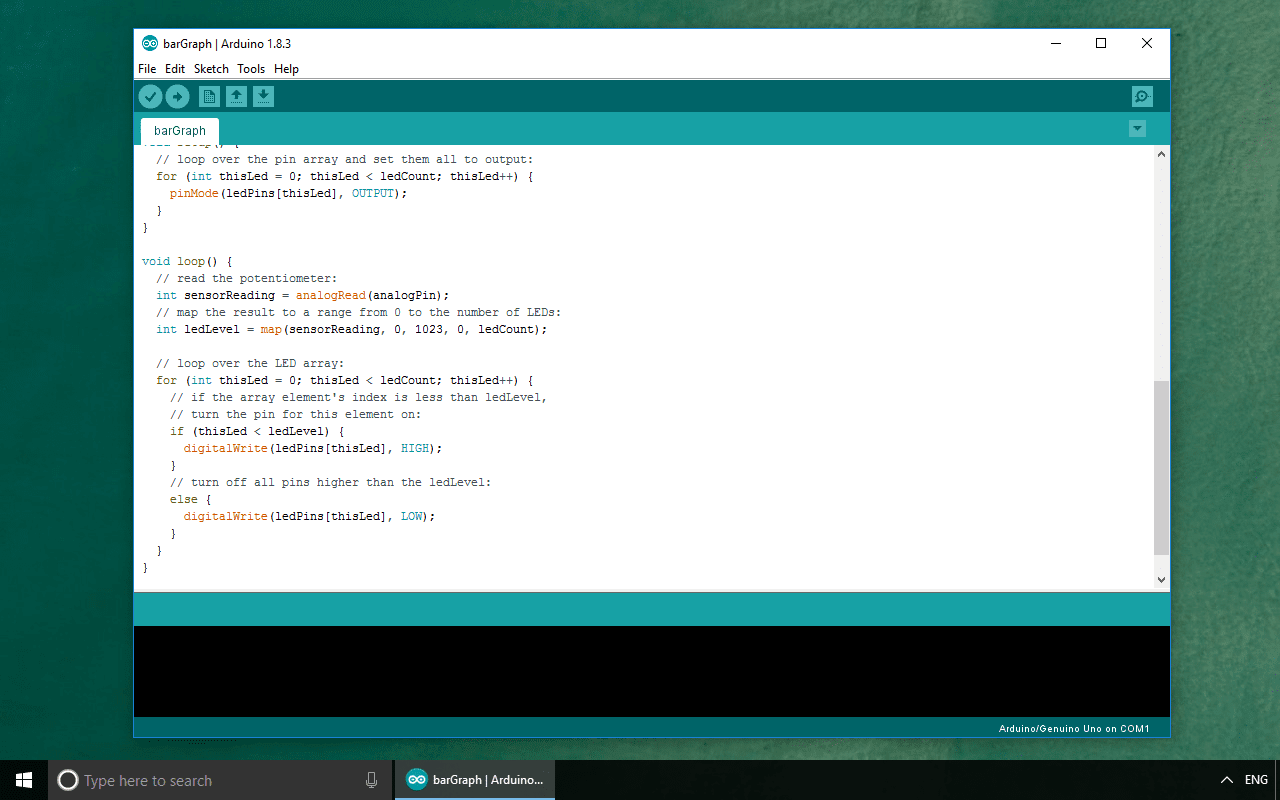
\includegraphics[height= 7cm, width=13cm]{project/images/ide}
  \caption{\textbf{Arduino Coding IDE}}
\end{figure}

\begin{lstlisting}
  #include <Keypad.h>
#include <LiquidCrystal.h>
#include<SoftwareSerial.h>;
SoftwareSerial gsm(2,3);
const int ldr_pin = A0;

const byte ROWS = 4; //four rows
const byte COLS = 4; //three columns
char keys[ROWS][COLS] = {
  {'1','2','3'},
  {'4','5','6'},
  {'7','8','9'},
  {'*','0','#'}
};
byte rowPins[ROWS] = {4,5,6,7}; //connect to the row pinouts of the keypad
byte colPins[COLS] = {8,9,10,11}; //connect to the column pinouts of the keypad
 
Keypad keypad = Keypad( makeKeymap(keys), rowPins, colPins, ROWS, COLS );
 

String password = "1234";
String mypassword;
 
int lock = 13;
 
int counter = 0; 
int attempts = 0; 
int max_attempts = 3; 
 
void setup(){
  Serial.begin(9600);
  // set up the LCD's number of columns and rows: 
 
  
 
  pinMode(lock, OUTPUT);
  pinMode(12,OUTPUT);
   pinMode(ldr_pin,INPUT);
  digitalWrite(12,HIGH);
 
  digitalWrite(lock, LOW);
  
  Serial.println("enter password");
    
}
  
void loop()
{
  
 keypadfunction();
 ldr();
 
}
 
void keypadfunction()
{
 char key = keypad.getKey();
  
  if (key){
    Serial.println(key);
    
  }
  if (key == '1')
  {
 
    mypassword = mypassword + 1;   
  }
  
    if (key == '2')
  {
 
    mypassword = mypassword + 2;  
  }
  
  if (key == '3')
  {
 
    mypassword = mypassword + 3; 
  }
  
   if (key == '4')
  {
  
    mypassword = mypassword + 4;  
  }
  
  if (key == '5')
  {
  
    mypassword = mypassword + 5;
  }
  
   if (key == '6')
  {
   
    mypassword = mypassword + 6; 
  }
  
   if (key == '7')
  {
 
    mypassword = mypassword + 7; 
  }
 
   if (key == '8')
  {
 
    mypassword = mypassword + 8; 
  }
  
  if (key == '9')
  {
 
    mypassword = mypassword + 9;
  }
             
                 if (key == '0')
  {
 
    mypassword = mypassword + 0; 
  }
  
  
        if (key == '*')
  {
    Serial.println(mypassword); 
    
if ( password == mypassword )
{
Serial.print(""); 
Serial.println("SYSTEM UNLOCKED");

Serial.println("WELCOME OWNER");
digitalWrite(lock, HIGH);
delay(50000                                                                                                                                               ); 
digitalWrite(lock,LOW);
mypassword = ""; 
counter = 0;  
Serial.println("Enter password");
}
else
{
Serial.println("wrong");

attempts = attempts + 1; 
if (attempts >= max_attempts )
{
  Serial.print("");
  call();
  digitalWrite(12,HIGH);
   
  Serial.print("Locked Out");
  

delay(5000); 
 
attempts = 0; 

}
mypassword = ""; 
counter = 0; 
Serial.print(""); 
 
Serial.print("Wrong Password");
delay(1000);

 
Serial.print("max attempts 3");
delay(1000);

Serial.print(""); 
Serial.println("Enter password");
 
}
    
  }  
  
  
}
void ldr()
{
  int ldrStatus = analogRead(ldr_pin);
  

if (ldrStatus <= 200) {

digitalWrite(12, LOW);


} else {
digitalWrite(12, HIGH);
call();
delay(5000);




}


  }
void call()
{
  gsm.begin(9600);
  gsm.println("ATD+918380843911;"); //replace x by your number
  delay(100);
  gsm.println("ATH");

  }
\end{lstlisting}
\newpage

